% ------ METADATA ------
\newcommand{\bookauthor}{\ml{$0$}{Эмиль~Весна}{Emil~Viesn\'{a}}}
\newcommand{\booktitle}{\ml{$0$}{ЛИСЬИ~СКАЗКИ}{Foxy~Tales}}
\newcommand{\bookstarted}{\ml{$0$}{28 мая 2023}{May 28, 2023}}
\newcommand{\bookfinished}{\ml{$0$}{пока нет}{not yet}}
% ------ METADATA ------

% ----- XELATEX SYMBOL -----
\usepackage{xltxtra}
% ----- XELATEX SYMBOL -----

% ----- HYPHENATION -----
\usepackage{hyphenat}
% ----- HYPHENATION -----

% ----- GEOMETRY -----
\usepackage[left=1.5cm,right=1.5cm,top=2cm,bottom=2cm,bindingoffset=0.5cm]{geometry}
% ----- GEOMETRY -----

% ----- INCLUDE PDF AS PAGES -----
\usepackage{pdfpages}
% ----- INCLUDE PDF AS PAGES -----

% ----- TOC CONFIG -----
\setcounter{tocdepth}{0}
\usepackage{titletoc}
\titlecontents{chapter}[0pt]{\large}%above code
{\MakeUppercase{\chaptername~\thecontentslabel}. }
{}%numberless chapter%
{\mdseries\titlerule*[0.75em]{.}\thecontentspage}
% ----- TOC CONFIG -----

% ----- DROPPING CAP -----
\usepackage{type1cm,lettrine}
% ----- DROPPING CAP -----

% ----- FONTS -----
\renewcommand{\baselinestretch}{1.2}
\setmainfont{Linux Libertine}
% ----- FONTS -----

% ------ HYPERLINKS ------
\usepackage{hyperref}
\definecolor{LinkColor}{HTML}{0969DA}
\hypersetup{colorlinks=true, linkcolor=LinkColor, citecolor=LinkColor, filecolor=LinkColor, urlcolor=LinkColor}
% ------ HYPERLINKS ------

% ------ FANCY PAGE STYLE ------
\setlength{\headheight}{15pt}
\usepackage{fancyhdr}
\pagestyle{fancy}
\fancyhead[LE,RO]{\thepage}
\fancyhead[LO]{{\small\textsc{\booktitle}}}
\fancyhead[RE]{{\small\textsc{\bookauthor}}}
\fancyfoot{}
    \fancypagestyle{plain}{
    \renewcommand{\headrulewidth}{0mm}
    \fancyhead{}
    \fancyfoot{}
}
% ------ FANCY PAGE STYLE ------

% ------ ELEMENTS ------
\newcommand{\asterism}{\vspace{1em}{\centering\Large\bfseries$\ast~\ast~\ast$\par}\vspace{1em}}
\newcommand{\textspace}{\vspace{1em}{\centering\Large\bfseries<\dots>\par}\vspace{1em}}
\newcommand{\FM}{\footnotemark}
\newcommand{\FA}[1]{\footnotetext{#1 \emph{\ml{$0$}{---~Прим.~авт.}{---~Author.}}}}
% ------ ELEMENTS ------

\begin{document}

% ----- FRONT COVER -----
%\includepdf[pages={1}]{\coverfrontfilename}
% ----- FRONT COVER -----

% ----- EMPTY PAGE -----
\newpage\thispagestyle{plain}~
% ----- EMPTY PAGE -----

% ------ TITLE PAGE ------
\begin{titlepage}
{
\centering
{~\par}
\vspace{0.25\textheight}
{\LARGE\bookauthor\par}
\vspace{1.3cm}
{\Huge\textbf{\booktitle}\par}
\vfill
{\includegraphics[width=6em]{\publisherlogofilename}\par}
}
\end{titlepage}
% ------ TITLE PAGE ------

% ----- TABLE OF CONTENTS -----
\tableofcontents
% ----- TABLE OF CONTENTS -----

\chapter{Дедко Репейко ищет домик}
 
Жил да был на Кудрявом болоте дедко Репейко.
Долго жил.
Белочек из трясин вытаскивал, мышкам дорогу показывал.
Валенки из мха валял, листьями подшивал, шубейку сам себе тополиным пухом подбивал, спал под кустами, пока молод был.
А как состарился --- мёрзнуть стал, покашливать.
И здоровье уже не то, и ноги уж не такие резвые, и руки сдают.

<<Найду себе домик>>, --- решил дедко Репейко.

Сказано --- сделано.
Поехал дедко Репейко через болота.
А ездил он по традиции своей семьи, как ещё его прабабушка, Ереперья Лопуховна, ездила.

Видит дедко --- лиса бежит.
Уцепится своей колючей бородой за лисью шерсть и висит.
А как захочет слезть:

<<Отцепи меня, лиса, --- кричит, --- моя остановка>>.

Ухватит его лиса зубищами, стянет со своей рыжей шубки и дальше бежит.
А дедко Репейко зайца ждёт, чтобы и на нём прокатиться.

Долго ли, коротко ли, добрался дедко Репейко до края Кудрявого болота.

\textspace

Как уснул богатырь, подкрался дедко к его коню и разговорился.

<<Не служи ему, конюшка, --- сказал.
--- Знаю я таких богатырей.
Мышей и белочек пугают только, когда болотами едут>>.

<<Да как же мне не служить, --- заплакал конь.
--- С малолетства я под богатырём.
Из рук его ел, в битву его возил.
Натерпелся страху.
Не проживу я на воле>>.

<<Я тебе покажу луга с вкусной травой, --- уговаривал дедко Репейко, --- водой родниковой напою, а зимой сена дам>>.

\textspace

Горностай надкусил ремешки --- и упала с коня сбруя.
Мышка подточила --- и развалились богатырские доспехи.

Проснулся богатырь.
Хвать за меч --- а меч-то и развалился.
Доспехи поправил --- кольчуга расползлась, со шлема заклёпки посыпались.
Коня хватился --- и конь убежал.
Так и пошел богатырь домой, бездоспешный и пеший.

% ----- INFO PAGE -----
\newpage\thispagestyle{plain}
{\centering

% ----- LICENSE SIGNS BLOCK -----

\includegraphics[width=2.5em]{cc.pdf}~
\includegraphics[width=2.5em]{by.pdf}
% ----- LICENSE SIGNS BLOCK -----

\vspace{0.2em}

% ----- LICENSE BLOCK -----
{\ml{$0$}{Данная книга распространяется под лицензией \textbf{CC~BY~4.0}.}{This book is distributed under the \textbf{CC~BY~4.0} license.}\par}
{\ml{$0$}{Подробнее о лицензии:}{Details:} \href{https://creativecommons.org/licenses/by/4.0/deed.ru}{creativecommons.org/licenses/by/4.0}\par}
% ----- LICENSE BLOCK -----

\vfill

% ----- AUTHOR AND TITLE -----
{\large\bookauthor\par}
\vspace{0.5em}
{\Large\textbf{\booktitle}\par}
% ----- AUTHOR AND TITLE -----

\vfill

% ----- BOOK INFO -----
{\ml{$0$}{Начато:}{Started:} \textit{\bookstarted}\par}
{\ml{$0$}{Последняя редакция:}{Latest revision:} \textit{\bookfinished}\par}
{\ml{$0$}{Подробнее о книге:}{The book details:} \href{https://github.com/regnveig/tofa}{github.com/regnveig/tofa}\par}
% ----- BOOK INFO -----

\vfill

% ----- DOCUMENT INFO -----
{\ml{$0$}{Дизайн обложки: \textit{Э.\,Весна}}{The cover design by E.\,Viesn\'a}\par}
{\ml{$0$}{Компьютерная вёрстка: \textit{Э.\,Весна}}{The computer layout by E.\,Viesn\'a}\par}
{\ml{$0$}{Создано с помощью \XeLaTeX}{Created with \XeLaTeX}\par}
% ----- DOCUMENT INFO -----

\vspace{0.5em}

% ----- PUBLISHER INFO -----
{\textbf{\ml{$0$}{Свободное издательство <<Цунами>>}{\textsc{Tsunami}, an independent publisher}}\par}
{\ml{$0$}{Томск 2023}{Tomsk 2023}\par}
% ----- PUBLISHER INFO -----

\vfill

% ----- QR CODES -----
{\hfill
\begin{minipage}[t]{0.25\textwidth}
{\centering
{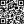
\includegraphics[width=0.8\textwidth]{qr_github_tofa.pdf}\par}
\vspace{0.2em}
{\small{\ml{$0$}{О книге и авторе}{About the book and the author}}\par}
}
\end{minipage}
\hspace{2em}
\begin{minipage}[t]{0.25\textwidth}
{\centering
{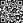
\includegraphics[width=0.8\textwidth]{qr_license_by40.pdf}\par}
\vspace{0.2em}
{\small{\ml{$0$}{Текст лицензии}{License full text}}\par}
}
\end{minipage}
\hfill}
% ----- QR CODES -----

}
% ----- INFO PAGE -----

% ----- BACK COVER -----
%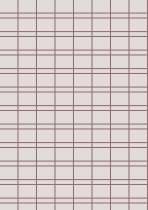
\includepdf[pages={1}]{cover_back.pdf}
% ----- BACK COVER -----

\end{document}
